\documentclass[12pt,twoside]{article}
%%%%%%%%%%%%%%%%%%%%%%%%%%%%%%%%%%%%%%%%%%%%%%%%%%%%%%%%%%%%%
% Meta informations:
\newcommand{\trauthor}{Horst Hansen}
\newcommand{\trtype}{Seminar Paper} %{Seminararbeit} %{Proseminararbeit}
\newcommand{\trcourse}{Knowledge Processing with Neural Networks}
\newcommand{\trtitle}{Neural Networks for Artificial Agents}
\newcommand{\trmatrikelnummer}{6543210}
\newcommand{\tremail}{hansen@informatik.uni-hamburg.de}
\newcommand{\trarbeitsbereich}{Knowledge Technology, WTM}
\newcommand{\trdate}{01.04.2014}

%%%%%%%%%%%%%%%%%%%%%%%%%%%%%%%%%%%%%%%%%%%%%%%%%%%%%%%%%%%%%
% Languages:

% Falls die Ausarbeitung in Deutsch erfolgt:
% \usepackage[german]{babel}
% \usepackage[T1]{fontenc}
% \usepackage[latin1]{inputenc}
% \usepackage[latin9]{inputenc}	 				
% \selectlanguage{german}

% If the thesis is written in English:
\usepackage[english]{babel} 						
\selectlanguage{english}

%%%%%%%%%%%%%%%%%%%%%%%%%%%%%%%%%%%%%%%%%%%%%%%%%%%%%%%%%%%%%
% Bind packages:
\usepackage{acronym}                    % Acronyms
\usepackage{algorithmic}								% Algorithms and Pseudocode
\usepackage{algorithm}									% Algorithms and Pseudocode
\usepackage{amsfonts}                   % AMS Math Packet (Fonts)
\usepackage{amsmath}                    % AMS Math Packet
\usepackage{amssymb}                    % Additional mathematical symbols
\usepackage{amsthm}
\usepackage{booktabs}                   % Nicer tables
%\usepackage[font=small,labelfont=bf]{caption} % Numbered captions for figures
\usepackage{color}                      % Enables defining of colors via \definecolor
\definecolor{uhhRed}{RGB}{254,0,0}		  % Official Uni Hamburg Red
\definecolor{uhhGrey}{RGB}{122,122,120} % Official Uni Hamburg Grey
\usepackage{fancybox}                   % Gleichungen einrahmen
\usepackage{fancyhdr}										% Packet for nicer headers
%\usepackage{fancyheadings}             % Nicer numbering of headlines

%\usepackage[outer=3.35cm]{geometry} 	  % Type area (size, margins...) !!!Release version
%\usepackage[outer=2.5cm]{geometry} 		% Type area (size, margins...) !!!Print version
%\usepackage{geometry} 									% Type area (size, margins...) !!!Proofread version
\usepackage[outer=3.15cm]{geometry} 	  % Type area (size, margins...) !!!Draft version
\geometry{a4paper,body={5.8in,9in}}

\usepackage{graphicx}                   % Inclusion of graphics
%\usepackage{latexsym}                  % Special symbols
\usepackage{longtable}									% Allow tables over several parges
\usepackage{listings}                   % Nicer source code listings
\usepackage{multicol}										% Content of a table over several columns
\usepackage{multirow}										% Content of a table over several rows
\usepackage{rotating}										% Alows to rotate text and objects
\usepackage[hang]{subfigure}            % Allows to use multiple (partial) figures in a fig
%\usepackage[font=footnotesize,labelfont=rm]{subfig}	% Pictures in a floating environment
\usepackage{tabularx}										% Tables with fixed width but variable rows
\usepackage{url,xspace,boxedminipage}   % Accurate display of URLs

%%%%%%%%%%%%%%%%%%%%%%%%%%%%%%%%%%%%%%%%%%%%%%%%%%%%%%%%%%%%%
% Configurationen:

\hyphenation{whe-ther} 									% Manually use: "\-" in a word: Staats\-ver\-trag

%\lstloadlanguages{C}                   % Set the default language for listings
\DeclareGraphicsExtensions{.pdf,.svg,.jpg,.png,.eps} % first try pdf, then eps, png and jpg
\graphicspath{{./src/}} 								% Path to a folder where all pictures are located
\pagestyle{fancy} 											% Use nicer header and footer

% Redefine the environments for floating objects:
\setcounter{topnumber}{3}
\setcounter{bottomnumber}{2}
\setcounter{totalnumber}{4}
\renewcommand{\topfraction}{0.9} 			  %Standard: 0.7
\renewcommand{\bottomfraction}{0.5}		  %Standard: 0.3
\renewcommand{\textfraction}{0.1}		  	%Standard: 0.2
\renewcommand{\floatpagefraction}{0.8} 	%Standard: 0.5

% Tables with a nicer padding:
\renewcommand{\arraystretch}{1.2}

%%%%%%%%%%%%%%%%%%%%%%%%%%%%
% Additional 'theorem' and 'definition' blocks:
\theoremstyle{plain}
\newtheorem{theorem}{Theorem}[section]
%\newtheorem{theorem}{Satz}[section]		% Wenn in Deutsch geschrieben wird.
\newtheorem{axiom}{Axiom}[section] 	
%\newtheorem{axiom}{Fakt}[chapter]			% Wenn in Deutsch geschrieben wird.
%Usage:%\begin{axiom}[optional description]%Main part%\end{fakt}

\theoremstyle{definition}
\newtheorem{definition}{Definition}[section]

%Additional types of axioms:
\newtheorem{lemma}[axiom]{Lemma}
\newtheorem{observation}[axiom]{Observation}

%Additional types of definitions:
\theoremstyle{remark}
%\newtheorem{remark}[definition]{Bemerkung} % Wenn in Deutsch geschrieben wird.
\newtheorem{remark}[definition]{Remark} 

%%%%%%%%%%%%%%%%%%%%%%%%%%%%
% Provides TODOs within the margin:
\newcommand{\TODO}[1]{\marginpar{\emph{\small{{\bf TODO: } #1}}}}

%%%%%%%%%%%%%%%%%%%%%%%%%%%%
% Abbreviations and mathematical symbols
\newcommand{\modd}{\text{ mod }}
\newcommand{\RS}{\mathbb{R}}
\newcommand{\NS}{\mathbb{N}}
\newcommand{\ZS}{\mathbb{Z}}
\newcommand{\dnormal}{\mathit{N}}
\newcommand{\duniform}{\mathit{U}}

\newcommand{\erdos}{Erd\H{o}s}
\newcommand{\renyi}{-R\'{e}nyi}
%%%%%%%%%%%%%%%%%%%%%%%%%%%%%%%%%%%%%%%%%%%%%%%%%%%%%%%%%%%%%
% Document:
\begin{document}
\renewcommand{\headheight}{14.5pt}

\fancyhead{}
\fancyhead[LE]{ \slshape \trauthor}
\fancyhead[LO]{}
\fancyhead[RE]{}
\fancyhead[RO]{ \slshape \trtitle}

%%%%%%%%%%%%%%%%%%%%%%%%%%%%
% Cover Header:
\begin{titlepage}
	\begin{flushleft}
		Universit\"at Hamburg\\
		Department Informatik\\
		\trarbeitsbereich\\
	\end{flushleft}
	\vspace{3.5cm}
	\begin{center}
		\huge \trtitle\\
	\end{center}
	\vspace{3.5cm}
	\begin{center}
		\normalsize\trtype\\
		[0.2cm]
		\Large\trcourse\\
		[1.5cm]
		\Large \trauthor\\
		[0.2cm]
		\normalsize Matr.Nr. \trmatrikelnummer\\
		[0.2cm]
		\normalsize\tremail\\
		[1.5cm]
		\Large \trdate
	\end{center}
	\vfill
\end{titlepage}

	%backsite of cover sheet is empty!
\thispagestyle{empty}
\hspace{1cm}
\newpage

%%%%%%%%%%%%%%%%%%%%%%%%%%%%
% Abstract:

% Abstract gives a brief summary of the main points of a paper:
\section*{Abstract}
  This paper gives a brief overview and an example of how to write a seminar paper in \LaTeX. Seminar papers are often seen as a review of an area research or as an overview over several approaches for a given problem. An ``Abstract'' serves as a complete summary and teaser of the paper: What is it all about? What is the open problem? What are possible solutions? What is the (abstract) result of this paper? --- Usually you (re-)write the Abstract as the last step of your paper writing.

% Lists:
\setcounter{tocdepth}{2} 					% depth of the table of contents (for Seminars 2 is recommented)
\tableofcontents
\pagenumbering{arabic}
\clearpage

%%%%%%%%%%%%%%%%%%%%%%%%%%%%
% Content:

% the actual content, usually separated over a number of sections
% each section is assigned a label, in order to be able to put a
% crossreference to it

\section{Introduction}
\label{sec:introduction}

The introduction motivates the research question. Ideally it describes the field, the specific open problem, why this is important, and -- most importantly -- what answer/approach/idea could possibly solve the problem. Keep in mind: Already in the introduction, every claim or idea that is not your (the author's) claim/idea needs a reference!

In addition, the introduction outlines the main ideas of the following paper and what are the main contributions of the paper. Remember: The main goal of the seminar paper is NOT to repeat the content of a textbook, but to provide an OWN view on different very recent solutions for an open problem.

If the paper has more than 4 pages, a reader's guide is recommenced. In a short paragraph an outline of the content of the next sections.

\section{Optional: Background Information}
\label{sec:basics}
A brief section giving background information may be absolutely necessary, especially if your work spans across two or more traditional fields. That means that your readers may not have any experience with some of the material needed to follow your paper, so you need to provide the most important foundations. A different title than that given above is usually better; e.g., "A Brief Review of Frammis Algebra."


\section{Models/Approaches/Methods Descriptions}
\label{sec:model}

After the (one or maybe two) common section(s) Introduction (and optional Background), more sections with the actual content of a paper follow. The style and structure of such sections varies by a large degree, no general rules of thumb can be given. However it is very important to describe each model/approach/method with respect to your research question: How can this model/approach/method solve the open question? 

All sources must be properly referenced, ideally by using the BiBTeX system. References can then be very conveniently made with the \textsc{cite} command. For example, reference
\cite{Leunen:Scholars:92} discusses some of the elementary rules on writing scientific papers, amongst others how to correctly cite other documents. Reference \cite{Taylor:SIGuide:95}, e.g., describes how to correctly use the SI system of units and their correct typographical
representation. In general you organise this section(s) by idea, and not by author or by publication.

For a good seminar paper you should end up having a number of approaches described that you can compare afterwards. Also in this section, the title of the section should be very meaningful and ideally name the proposed model/approach/method.

\subsection{Word processing with \LaTeX}
\label{sec:model:subsec:latex}

This document already has introduced the most important constructs of \LaTeX. What is necessary to produce documents with \LaTeX is simple any normal text editor and a \LaTeX distribution. This is commonly installed on practically all UNIX-type systems; for Windows, an
excellent \LaTeX exists, called MikTeX, available from \url{www.miktex.org}. Almost all distributions come with a large patch of examples and introductory material; consult your local installation for details. 

Lots of supplementary and background information, FAQs, etc.\ is available from the Comprehensive TeX Archive Network (CTAN); the German mirror of which is \url{www.dante.de}. 

\subsection{Tables in \LaTeX}
\label{sec:model:subsec:tables}
Tables should be centred and should always have a caption positioned above it. A caption in a sentence form as well as in a short form must end with a period as seen in table~\ref{tab:sample}. Ideally the table can be understood sorely by the table and the caption itself. The parameters ``hbtp'' provide a list of priorities for the arrangement of the table: here, bottom, top, (next) page.

\begin{table}[hbtp] 
  \caption{This caption has one line so it is centred.}\label{tab:sample} 
  \centering
  \begin{tabular}{|c|c|}
    \hline
    Example column 1 & Example column 2 \\
    \hline
    Example text 1 & Example text 2 \\
    \hline
  \end{tabular}
\end{table}

\subsection{Figures in \LaTeX}
\label{sec:model:subsec:figures}
Note that a figure is a so-called floating object: it is moved around the actual text in order to best fit on a page. This is in strong contrast to some GUI-based word processing tools, where the placement of figures is usually more associated with luck than principle.

As figures float around, expressions like ``the following figure'' must never be used. Instead, figures need a caption, a label, and must be properly referenced in the main text. A figure caption is placed centred below the figure and describes the figure in (very) short. Again, ideally the figure can be understood sorely by the figure and the caption itself.

In general, only vector graphics in encapsulated postscript (EPS) or a similar format (SVG, PDF) should be included in any kind of text, as this allows arbitrary scaling, rotation etc.\ without any loss of quality. Bitmap formats (JPEG, GIF, \dots) should only be used if no other alternative exists --- basically the only case where bitmaps can be justified is when scanned pictures need to be included in a text, however, this should be avoided as hard as possible as the quality in usually not satisfactory. If a screen shot is needed a high resolution picture without visible fragments of a jpeg compression is allowed. Figures like the figure~\ref{fig:samplefig} (this is how you refer to figures correctly!) should always appear after the first referencing it.
\begin{figure}[hbtp]
	 \centerline{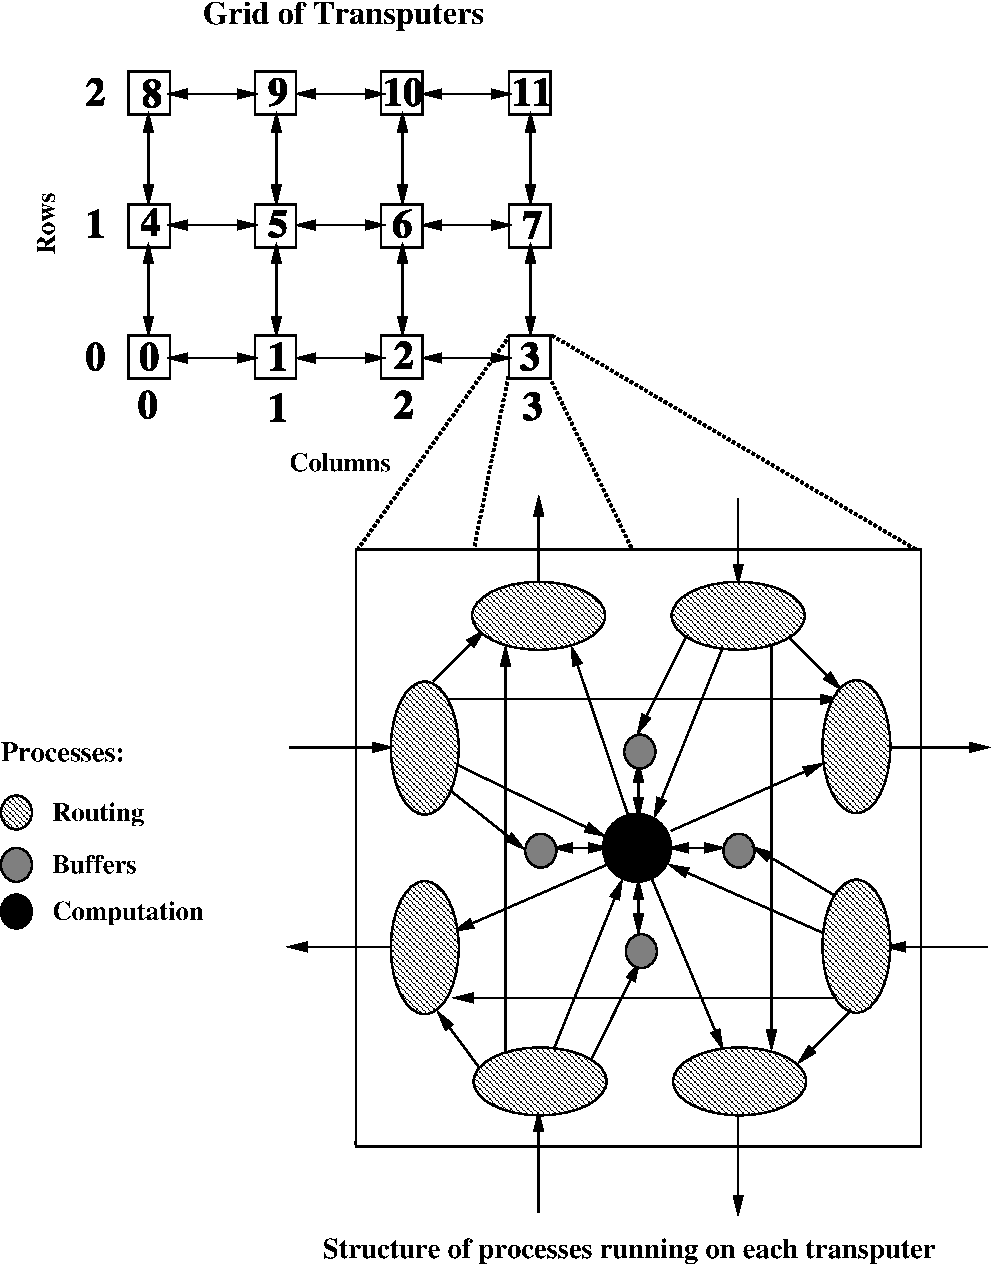
\includegraphics[width=0.6\textwidth]{samplefig.pdf}}
	 {\caption{Network of transputers and the structure of individual
processes.}\label{fig:samplefig}}
\end{figure}

\section{Models/Approaches/Methods Analysis \\ and Comparison}
\label{sec:analysis}
The analysis the proposed models/approaches/methods descriptions is a much more free-form of a paper. Starting with a comparison of several approaches over some experimental settings and result up to a theoretical verification of the model(s), anything is allowed. But it all should only serve one purpose: to convince the reader of the right to exist of the described models/Approaches/methods. For a seminar paper this is the most important section and your (the author's) own contribution!

\section{Conclusion}
\label{sec:concl}

At the end, there is a final section concluding and summarizing a paper, putting the entire work into perspective and explaining, on a larger level, what the consequence of the models/approaches/methods are and how this answers the research question that has been raised in the introduction. Also, unexpected results can be discussed here, etc.

%%%%%%%%%%%%%%%%%%%%%%%%%%%%%%%%%%%%%%
% hier werden - zum Ende des Textes - die bibliographischen Referenzen
% eingebunden
%
% Insbesondere stehen die eigentlichen Informationen in der Datei
% ``bib.bib''
%
\newpage
\bibliographystyle{plain}
\addcontentsline{toc}{section}{Bibliography}% Add to the TOC
\bibliography{bib}

\end{document}


